% !TeX spellcheck = en_GB
\documentclass[10pt,letterpaper,oneside]{article}
\usepackage{fontspec}
\usepackage{arev}
\usepackage[utf8]{inputenc}
\usepackage[T1]{fontenc}
\usepackage{amsmath}
\usepackage{amsfonts}
\usepackage{amssymb}
\usepackage{graphicx}
\usepackage{csquotes}
\usepackage{booktabs}
\usepackage{multicol}
\usepackage{enumerate}
\usepackage{microtype}
\usepackage[labelfont=bf,font={small}]{caption}
\usepackage{hyperref}
\usepackage{booktabs}
\usepackage{subcaption}
\usepackage{fancyhdr}
\usepackage[svgnames]{xcolor}
\usepackage{mdframed}
\usepackage{multicol}
\usepackage[para]{footmisc}
\usepackage{siunitx}
\usepackage{cleveref}
\usepackage{listings}
\usepackage{cprotect}


\lstset{ % General setup for the package
	language=Python,
	basicstyle=\small\ttfamily,
	tabsize=4,
	columns=fixed,
	showstringspaces=false,
	showtabs=false,
	keepspaces,
	commentstyle=\color{SeaGreen},
	keywordstyle=\bf\ttfamily\color{DarkBlue},
	stringstyle=\ttfamily\color{Crimson}
}

\newfontfamily\symbolfont{Symbola}
\usepackage[left=1in,right=1in,top=1in,bottom=1in,marginparwidth=0.3in]{geometry}

\usepackage[sorting=none]{biblatex}
\addbibresource{../bibliography.bib}

\author{Andreas Stöckel\\[0.5cm]Based on lecture notes by\\Chris Eliasmith and Terrence~C.~Stewart}
\newcommand{\baseCodeURL}{https://github.com/celiasmith/syde556-w22/blob/master/lectures}

\fancyhf{}
\fancyhead[L]{SYDE 556/750 Lecture Notes}
\fancyhead[R]{Andreas Stöckel}
\fancyfoot[C]{\thepage}
\pagestyle{fancy}

\setlength{\parindent}{0em}
\setlength{\parskip}{0.5em}
\renewcommand{\baselinestretch}{1.25}

\renewcommand{\vec}[1]{{\mathbf{#1}}}
\newcommand{\mat}[1]{{\mathbf{#1}}}
\newcommand{\T}{\ensuremath{\mathrm{T}}}
\renewcommand{\epsilon}{\varepsilon}
\renewcommand{\phi}{\varphi}

\makeatletter
\newcommand{\superimpose}[2]{%
	{\ooalign{{#1}\hidewidth\cr{#2}\hidewidth\cr}}}
\makeatother
\newcommand{\SolidCircle}[2]{\superimpose{\color{#1}\symbolfont ⬤}{\textbf{\color{white}#2}}\hspace{1em}}
\newcommand{\OPlus}{\SolidCircle{DarkGreen}{\kern0.75pt+}}
\newcommand{\OMeh}{\SolidCircle{DarkOrange}{~}}
\newcommand{\OMinus}{\SolidCircle{DarkRed}{\kern2.25pt--}}

\newcommand{\YouTube}[2][Video]{\href{https://youtu.be/#2}{{\symbolfont 📺}~{#1}}%
%\footnote{\url{https://youtu.be/#2}}%
}

\newcommand{\CodeLink}[2][Code]{\href{\baseCodeURL/#2}{{\symbolfont ⌨}~\emph{#1}}}

\newcommand{\MakeTitle}[1]{
\maketitle
\begin{center}
	\includegraphics[width=0.5\textwidth]{../assets/uwlogo.pdf}\\[1cm]
	{#1}\
\end{center}

\vfill

\thispagestyle{empty}
\setcounter{page}{0}
\newpage

\pagenumbering{roman}
\setcounter{tocdepth}{2}
\tableofcontents
\newpage

\setcounter{page}{0}
\pagenumbering{arabic}}

\reversemarginpar


\newcommand{\ColorBox}[3]{%
	\marginpar{%
		\huge\raisebox{-3ex}{\symbolfont{#1}}%
	}%
	\begin{mdframed}[hidealllines=true,backgroundcolor=#2,innertopmargin=0.25cm,innerbottommargin=0.25cm]%
		{#3}
	\end{mdframed}}

\newcommand{\Note}[1]{\ColorBox{📌}{WhiteSmoke}{\textbf{Note:} #1}}
\newcommand{\Example}[1]{\ColorBox{💡}{WhiteSmoke}{\textbf{Example:} #1}}
\newcommand{\Aside}[1]{\ColorBox{🌟}{WhiteSmoke}{\emph{Aside:} #1}}
\newcommand{\Python}[1]{\ColorBox{🐍}{WhiteSmoke}{#1}}
\newcommand{\Notation}[1]{\ColorBox{\huge$\Sigma$}{WhiteSmoke}{\textbf{Notaton:} #1}}

\newcommand{\ConstructionSite}{\hrulefill {\symbolfont 🚧} UNDER CONSTRUCTION {\symbolfont 🚧} \hrulefill}

\newenvironment{ImportantEqn}[1]{\mdframed\raggedleft\emph{({#1})}\align}{\endalign\endmdframed}

\date{November 4, 2022}
\title{SYDE 556/750 \\ Simulating Neurobiological Systems \\ Lecture 9: Analysing Representation}


\begin{document}

\MakeTitle{\textbf{Accompanying Readings: Chapter 7 of Neural Engineering}}



\begin{itemize}
	\item \textbf{Observation:} Some functions are \enquote{harder} to decode than others (larger error)
	\item \textbf{Goal:} Get a better understanding of the types of function that can be decoded
	\item Tuning curves are a set of basis functions; decoders combine these basis functions
	\begin{align*}
		\hat x &= \sum_{i = 1}^n d_i a_i(x) = \langle \vec d, \vec a(x) \rangle
	\end{align*}
	\item Tuning curves are highly similar
	\item Find basis transformation $\mat T$ that maximises the information in the basis functions $\Rightarrow$ PCA
	\begin{align*}
		\hat x &= \langle \vec d, \mat T \vec a \rangle = \langle \vec d \mat T^{-1}, \mat T \vec a \rangle
	\end{align*}
	\item The scale of Eigenvalues corresponding to the individual Principal Compnents is inversely proportional to the noise in the decoding. So if a component has a large Eigenvalue $\Rightarrow$ this basis function can be decoded well
\end{itemize}

\section{Introduction}

Recall that we can write our estimate of $\mathbf{X}$ in matrix notation:
\begin{eqnarray*}
  \hat{\mathbf{X}} & = & \mathbf{A}\mathbf{D}\\
   & = & \mathbf{A}(\mathbf{A}^{T}\mathbf{A})^{-1}\mathbf{A}^{T}\mathbf{X}.
\end{eqnarray*}

We have used packages that take the inverse of $\gamma = \mathbf{A}^{T}\mathbf{A}$ `in the right way'. However, because this matrix has no noise term, and because \emph{some} tuning curves are likely to be similar for a large population, that Gram matrix is likely to be singular, or nearly singular
so it is \emph{not} invertible. As we have previously seen, there exists a general, and very powerful, technique for analyzing
such singular matrices called singular value decomposition (SVD).
Recall that SVD decomposition of an $M\times N$ matrix, $\mathbf{B}$, results in three matrices whose product gives $\mathbf{B}$, i.e.,
\[
\mathbf{B}_{M\times N}=\mathbf{U}_{M\times N}\mathbf{S}_{N\times N}\mathbf{V}_{N\times N}^{T}.
\]
The matrix $\mathbf{S}$ is a diagonal matrix whose entries are called
the \emph{singular values} of $\mathbf{B}$. In the case when $\mathbf{B}$ is square and symmetrical (as with our example), this simplifies to
\begin{eqnarray*}
\boldsymbol{\gamma} & = & \mathbf{USU}^{T}.
\end{eqnarray*}

\section{Singular Value Decomposition of $\mathbf{A}$}

In the case where $\gamma$ is singular (or nearly so), some elements
of $\mathbf{S}$ are zero (or very small), so the inverse of $\mathbf{S}$
includes infinite (or very large) terms, meaning the inverse of $\gamma$
is ill-defined (as expected for singular or near singular matrices).
In this case, the SVD `pseudo-inverse' is defined where for $S_{i}=0$,
the inverse is set to $0$. The methods we call for inverting matrices do this 'automatically' (or we add noise to make them invertible). Interestingly, even in the case when a matrix is singular (or nearly so), SVD can
be very informative. The columns of $\mathbf{U}$ whose corresponding
singular values are non-zero form an orthonormal basis that spans
the range and the corresponding zero elements form an orthonormal
basis that spans the null space.


This decomposition is useful for characterizing representation and
transformation for a number of reasons. 
\begin{itemize}
\item First, as already mentioned, the relevant $\mathbf{U}$ matrix provides
an orthogonal basis for both the range and nullity of $\boldsymbol{\gamma}$.
Because $\boldsymbol{\gamma}$ tends to be singular, both bases are
important. 
\item Second, when a vector in $\Upsilon$ lies in the range of $\boldsymbol{\gamma}$,
the SVD pseudo-inverse guarantees that the corresponding vector from
$\mathbf{D}$ \emph{minimizes}
the length of that $\mathbf{D}$ vector. This is important
because given that $\boldsymbol{\gamma}$ is singular, there are an
infinite number of solutions for $\mathbf{D}$. The solution
that provides the shortest vector is a natural and compact choice
from the set. 
\item Third, when a vector in $\Upsilon$ lies in the nullity of $\boldsymbol{\gamma}$,
the SVD pseudo-inverse guarantees that the best (in the least squares
sense) $\mathbf{D}$ given $\Upsilon$ will be found. In other
words, this `pseudo-inverse' minimizes the error. Thus, we can use
SVD to find the optimal decoding functions, which we can now write
as
\begin{equation}
  \mathbf{D}=\mathbf{US}^{-1}\mathbf{U}^{T}\mathbf{A}^{T}\mathbf{X}.\label{c4.eq.phi.svd}
\end{equation}
Given the properties of SVD, we know that this is the same solution
we would find by constructing the error explicitly (i.e., $E=\left\langle \left[\mathbf{X}-\hat{\mathbf{X}}\right]^{2}\right\rangle _{\mathbf{X}}$),
taking the derivative, and setting it to zero, as we have previously
done. 
\end{itemize}

Recall that regardless of which transformation we need decoders for,
we always perform SVD on the same matrix, $\gamma=\mathbf{A}^{T}\mathbf{A}$.
This suggests that understanding the properties of $\gamma$ can provide
general insight into all possible decodings of the population, $a_{i}$. 

The singular values are useful because they tell us the \emph{importance}
of the corresponding $\mathbf{U}$ vector. There are a number of ways
of thinking about `importance' in this case. 

\begin{itemize}
\item related to the error that would result if we left a particular vector
out of the mapping. 
\item related to the variance of population firing along the vectors in
the $\gamma$ matrix. 
\item being the amount of (independent) information about changes in population
firing that can be extracted by looking only at data projected onto
the corresponding $\mathbf{U}$ vector.
\item In general, we can think of the magnitude of the singular value as
telling us how relevant the dimension defined by the corresponding
$\mathbf{U}$ vector is to the identity of the matrix we have decomposed.
Since the matrix we have decomposed is like the correlation matrix
of the neuron tuning curves, the large singular values are most important
for accounting for the structure of those correlations. 
\end{itemize}

Notice also that the vectors in $\mathbf{U}$ are orthogonal: they
provide an (ordered) orthogonal \emph{basis} for that matrix. This
is very useful because the original \textbf{$\gamma$} matrix was
generated by a non-ordered non-orthogonal basis; the neuron tuning
curves. 

To dive in a bit more, define a point in the `neuron space' (i.e., the
space spanned by the overcomplete neuron tuning curves) as
\[
\mathbf{a}=a_{1}\mathbf{e}_{1}+a_{2}\mathbf{e}_{2}+\ldots+a_{N}\mathbf{e}_{N}.
\]
In this notation, the vectors $\mathbf{e}_{i}$ serve as axes for
the state space of the neural population. A point in this space is
defined by the neuron firing rates from each neuron in the population
(which, taken together, form the vector $\mathbf{a}$). 

Because the neural responses are non-independently driven by some
variable, $\mathbf{x}$, only a \emph{subspace} of the space spanned
by the $\mathbf{e}_{i}$ vectors is ever \emph{actually} occupied
by the population.

The $\gamma$ matrix, because it tells us the correlations between
all neurons in the population, provides us with the information we
need to determine what that subspace is. When we find the $\mathbf{U}$
vectors in the SVD decomposition, we have characterized that subspace
because those are the orthogonal vectors that span it. 

Let's see how we can use this to determine what functions can be computed
by the particular encoding of $\mathbf{x}$ found in the $a_{i}$
population: 
\[
\hat{\mathbf{X}}=\mathbf{AUS}^{-1}\mathbf{U}^{T}\mathbf{A}^{T}\mathbf{X},
\]
 or, more simply
\begin{equation}
\hat{\mathbf{X}}=\chi\Phi,\label{c4.eq.chi.phi}
\end{equation}
 where 
\[
\chi=\mathbf{AU},
\]
and
\begin{eqnarray*}
\Phi & = & \mathbf{S}^{-1}\mathbf{U}^{T}\mathbf{A}^{T}\mathbf{X}\\
 & = & \mathbf{U}^{T}\mathbf{US}^{-1}\mathbf{U}^{T}\mathbf{A}^{T}\mathbf{X}\\
 & = & \mathbf{U}^{T}\mathbf{D},
\end{eqnarray*}
 
Notice that $\chi$ and $\Phi$ in (\ref{c4.eq.chi.phi}) are rotated
versions of $\mathbf{A}$ and $\mathbf{D}$ respectively. Specifically,
they are rotated into the coordinate system defined by $\mathbf{U}$.
So we can think of $\mathbf{U}$ as the rotation matrix that aligns
the first axis of the coordinate system along the dimension with the
greatest variance in the encoding of $\mathbf{x}$, the second axis
along the dimension with the second greatest variance, and so on.
As a result, the $\chi$
vectors also end up being orthogonal and ordered by importance. That
is, they tell us what can be extracted, and how well it can be extracted,
from the neural population. Figure \ref{svd.projection} shows an example of how the singular values can be seen as projections of some subspace in the neuron space.

\begin{figure}[h]
  \centering
  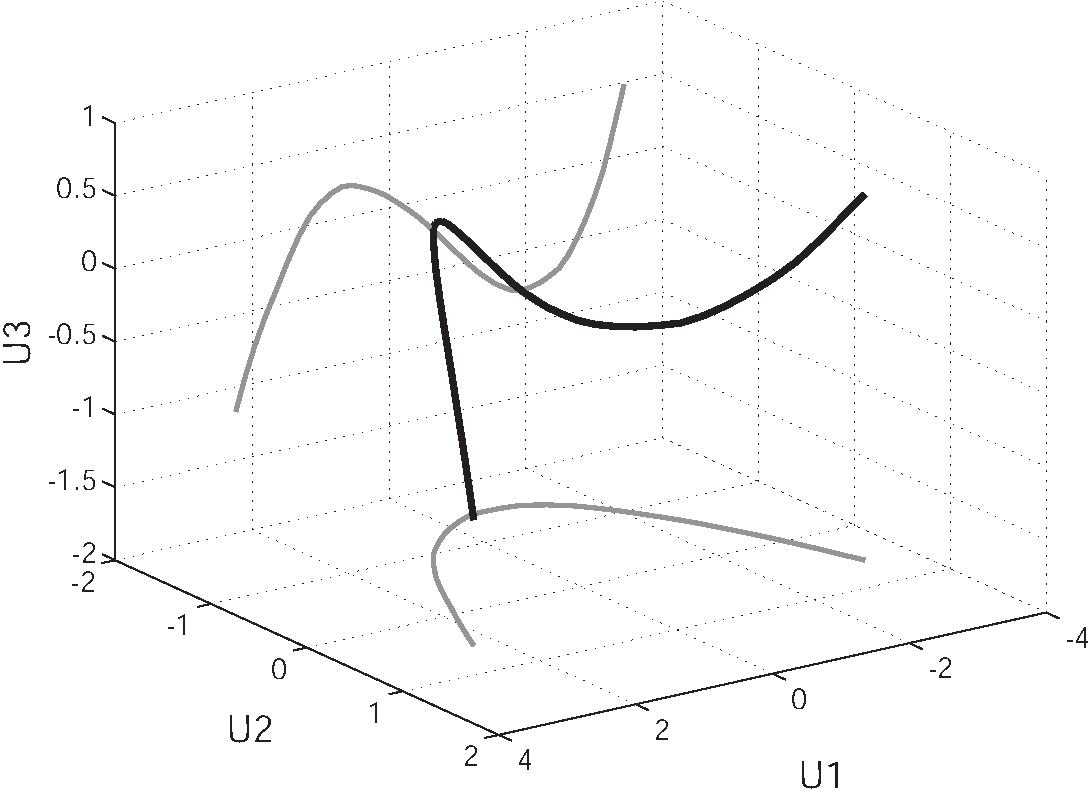
\includegraphics[scale=0.5]{media/c5.chi.projections.pdf}
  \caption{A subspace of neuron activity being projected onto the first few principle component planes. Notice that the axis scales are different, capturing the size of the singular value.}
	\label{svd.projection}
\end{figure}

We can think of the components of $\chi$ as \emph{basis
functions} of the space that includes the ensemble of transformations
definable on $\mathbf{x}$ using the encoding in the population $a_{i}$.Whichever $\chi(\mathbf{x})$ functions have reasonably large associated
singular values, are exactly the functions that we can do a good job
of extracting from our encoding of the input space, $\mathbf{x}$.
Of course, we can also extract any linear combinations of those $\chi(\mathbf{x})$
functions quite well. But, because these functions are ordered, the
more useful the `first' $\chi(\mathbf{x})$ function is for reconstructing
some transformation, $f(\mathbf{x})$, the better we can extract that
transformation, $f(\mathbf{x})$.

In practice, we can look at the resulting $\chi(\mathbf{x})$ functions
and determine what sort of basis we seem to have (see the many examples in the slides). Figure \ref{lif.pca} shows an example of doing this for LIF neuron tuning curves in 1D.

\begin{figure}[t]
  \centering
  \includegraphics{media/tuning_curve_lif_pca.pdf}
  \caption{The first few basis functions found from SVD of the activity correlation matrix.}
	\label{lif.pca}
\end{figure}

\section{Function bases and tuning curves}

When we do this to standard NEF 1D tuning curves, we approximately find one of the most common polynomial bases
used in mathematics, the Legendre basis,
$l_{i}(x)$, which is defined over the interval {[}-1,1{]} and results
from the orthogonalization of $x^{n}$.\footnote{One way of expressing the basis is: $l_{i}(x)=\frac{(-1)^{i}}{2^{i}i!}\frac{d^{i}}{dx^{i}}\left[\left(1-x^{2}\right)^{i}\right]$.}
Scaled versions of the first five elements of this basis are plotted
in figure \ref{c5.fig.broad.chi}. 

\begin{figure}[t]
  \centering
  \includegraphics{media/legendre.pdf}
  \caption{The first few Legendre Polynomials for comparison to those found from SVD of the activity correlation matrix.}
	\label{c5.fig.broad.chi}
\end{figure}

The similarity between $\chi_{m}(x)$ and $l_{i}(x)$ means that this
neural population supports the extraction of functions that can be
well-estimated using the standard Legendre basis. But the $\chi_{m}(x)$
functions are ordered by their singular values. Thus, the higher-order
polynomial terms are not as well encoded by our population as the
lower-order ones. So, computing functions that depend strongly on
precise high-order terms will be prone to error.

This is a natural basis to be found from the tuning curves in the
linear population. The tuning curves are very broad, and the polynomial
basis is also very broad. These tuning curves are approximately linear,
and the more linear basis functions are also the first ones. The Legendre
polynomial basis is ordered by decreasing linearity so it should not
be too surprising that this population supports the functions in precisely
that order. 

However, none of this would be true if the population did not do a
good job of evenly tiling the input space (see slides for examples). If, for example, there
were only high gain neurons, whose slopes were the same sign as their
$x$-intercepts (i.e., if the `on' and `off' sub-populations were
`clumped' near $x_{max}$ and $x_{min}$ respectively), we would not
expect the linear term to be better supported than the quadratic term.
In this sense, the heterogeneity of the population helps it support
the more natural ordering of the polynomial basis; clumping would
defeat this ordering. Thus, this particular set of $\chi_{m}(x)$
functions does not just depend on the general `shape' of the neuron
tuning curves, but also on which neurons are included in a population,
i.e., the degree of heterogeneity.

\subsection{Singular Values of Vector Representations}

There are additional analyses we can perform for vectors
of two or more dimensions. As shown in the slides, the same SVD analysis shows that 2D polynomials acts as a useful basis. However, when computing transformations of populations encoding $n$-dimensional
vectors, we must realize that there are additional cross terms (e.g.,
$x_{1}x_{2}$) that introduce variations in the encoding that are
not present in scalar transformations. The expansions are now of the
form
\begin{eqnarray*}
f(\mathbf{x}) & = & c_{0}+c_{1}x_{1}+c_{2}x_{2}+c_{3}x_{1}^{2}+c_{4}x_{2}^{2}+c_{5}x_{1}x_{2}+\ldots\\
 & = & \sum_{l=0}^{N_{order}}\sum_{n=0}^{l}c_{n,l-n}x_{1}^{n}x_{2}^{l-n},
\end{eqnarray*}
 where $N_{order}$ is the highest order term in the transformation
and $l$ indexes the $l$th order terms in the expansion (all terms
whose exponents \emph{sum} to $l$ are considered $l$th order terms).
As we can see, the cross terms (i.e., $x_{1}^{n}x_{2}^{l-n}$) are
quite common. In order to characterize how well an arbitrary function
can be decoded from a representation of $\mathbf{x}$, we need to
know how big the singular values of these cross terms are as well.

A quick inspection of the singular values of the population reveals
that all terms of a given order have singular values of approximately
the same magnitude (see Figure \ref{2d.singular.values}).

\begin{figure}[t]
  \centering
  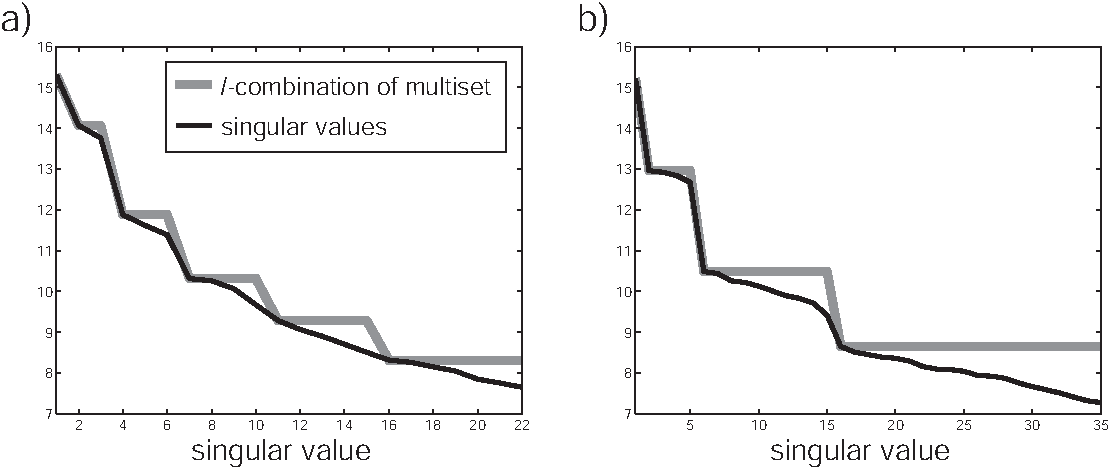
\includegraphics{media/c5.multiset.2D.pdf}
  \caption{The a) 2D and b) 4D singular values compared to the multiset prediction of how many cross terms there are.}
	\label{2d.singular.values}
\end{figure}

But there is an exponential decay in the magnitude of the singular
values as a function of the order of the polynomial. This means that
lower-order functions are \emph{significantly} better supported by
these kinds of broadly tuned neural populations. That is, the ability
to extract higher-order functions drops more quickly with an increase
in the order of the function than compared to the scalar case.

In fact, we can determine exactly how many singular values, $N_{S}$,
there should be for each order, $l$, in the polynomial for a input
space of size $D$ by using the equation for determining $l$-combinations
of a multi-set:
\begin{equation}
N_{S}(l,D)=\frac{(l+D-1)!}{l!(D-1)!}.\label{c5.eq.combinations}
\end{equation}

\section{Noise}

We have been ignoring noise, but most everything stays the same. Rather
than the encoding defining a precise subspace (the black line in Figure \ref{svd.projection}), we can think of it as defining a cloud (e.g. a
tube in Figure \ref{svd.projection}).

However, the noise does not scale with the singular values, it is isometric
in the vector space. This means that small singular values are more
greatly affected by noise. We can derive this.

We know the error with noise can be written in the vector case as
\begin{eqnarray}
E & = & \left\langle \left[\mathbf{x}-\sum_{i}\left(a_{i}(\mathbf{x})+\eta_{i}\right)\mathbf{d}_{i}\right]^{2}\right\rangle _{\mathbf{x},\eta}\nonumber \\
 & = & \left\langle \left[\mathbf{x}-\sum_{i}a_{i}(\mathbf{x})\mathbf{d}_{i}\right]^{2}+\sigma_{\eta}^{2}\sum_{i}\mathbf{d}_{i}^{2}\right\rangle _{\mathbf{x}}.\label{AH.eq.error}
\end{eqnarray}

We can now use our SVD expressions to give:
\begin{eqnarray}
E & = & \left\langle \left[\mathbf{x}-\sum_{m}\chi_{m}\Phi_{m}\right]^{2}+\sigma_{\eta}^{2}\sum_{i,j}\mathbf{d}_{i}\delta_{ij}\mathbf{d}_{j}\right\rangle _{\mathbf{x}}\nonumber \\
 & = & \left\langle \left[\mathbf{x}-\sum_{m}\chi_{m}\Phi_{m}\right]^{2}+\sigma_{\eta}^{2}\sum_{i,j}\mathbf{d}_{i}\sum_{m}U_{im}U_{mj}\mathbf{d}_{j}\right\rangle _{\mathbf{x}}\nonumber \\
 & = & \left\langle \left[\mathbf{x}-\sum_{m}\chi_{m}\Phi_{m}\right]^{2}+\sigma_{\eta}^{2}\sum_{m}\Phi_{m}^{2}\right\rangle _{\mathbf{x}}.\label{AH.eq.error.final}
\end{eqnarray}

We minimize this error by taking the derivative of (\ref{AH.eq.error.final})
and setting it to zero to get an expression for the optimal $\Phi$
functions under noise: 

\begin{eqnarray}
\frac{dE}{d\Phi_{n}} & = & \left\langle 2\left[\mathbf{x}-\sum_{m}\chi_{m}\Phi_{m}\right](-\chi_{n})+2\sigma_{\eta}^{2}\Phi_{n}\right\rangle _{\mathbf{x}}\nonumber \\
0 & = & -2\left\langle \chi_{n}\mathbf{x}\right\rangle _{\mathbf{x}}+2\left\langle \sum_{m}\chi_{m}\chi_{n}\Phi_{n}\right\rangle _{\mathbf{x}}+2\sigma_{\eta}^{2}\Phi_{n}\nonumber \\
\left\langle \chi_{n}\mathbf{x}\right\rangle _{\mathbf{x}} & = & S_{n}\Phi_{n}+\sigma_{\eta}^{2}\Phi_{n}\nonumber \\
\Phi_{n} & = & \frac{\left\langle \chi_{n}\mathbf{x}\right\rangle _{\mathbf{x}}}{S_{n}+\sigma_{\eta}^{2}}.\label{AH.eq.Phi2}
\end{eqnarray}

Note that $\sum_m \chi_m \chi_n = S_n$ because the $\chi$ are orthogonal, so only the $n_{th}$ term is non-zero. Furthermore, 
\begin{eqnarray*}
  \mathbf{\chi}^T \mathbf{\chi} &=& \mathbf{U}^T \mathbf{A}^T \mathbf{A} \mathbf{U} \\
  &=& \mathbf{U}^T \mathbf{U} \mathbf{S} \mathbf{U}^T \mathbf{U} \\
  &=& \mathbf{S}
\end{eqnarray*}

We can use this expression to determine what the residual error will
be (i.e., the expected error using these $\Phi$ functions). We can now determine the residual error as follows:
\begin{eqnarray*}
E_{r} & = & \left\langle \left[\mathbf{x}-\hat{\mathbf{x}}\right]^{2}\right\rangle _{\mathbf{x},\eta}\\
 & = & \left\langle \left[\mathbf{x}-\sum_{m}\chi_{m}\Phi_{m}\right]^{2}\right\rangle _{\mathbf{x},\eta}\\
 & = & \left\langle \mathbf{x}^{2}\right\rangle _{\mathbf{x},\eta}-2\left\langle \mathbf{x}\sum_{m}\chi_{m}\Phi_{m}\right\rangle _{\mathbf{x},\eta}+\left\langle \sum_{m}\chi_{m}\Phi_{m}\right\rangle _{\mathbf{x},\eta}^{2}.
\end{eqnarray*}

Substituting the expression in (\ref{AH.eq.Phi2}) for $\Phi_{m}$
gives:
\begin{eqnarray*}
E_{r} & = & \left\langle \mathbf{x}^{2}\right\rangle _{\mathbf{x},\eta}-2\left\langle \mathbf{x}\sum_{m}\chi_{m}\frac{\left\langle \chi_{m}\mathbf{x}\right\rangle _{\mathbf{x}}}{S_{m}+\sigma_{\eta}^{2}}\right\rangle _{\mathbf{x},\eta}+\left\langle \sum_{m}\chi_{m}\frac{\left\langle \chi_{m}\mathbf{x}\right\rangle _{\mathbf{x}}}{S_{m}+\sigma_{\eta}^{2}}\right\rangle _{\mathbf{x},\eta}^{2}\\
 & = & \left\langle \mathbf{x}^{2}\right\rangle _{\mathbf{x}}-2\sum_{m}\frac{\left\langle \chi_{m}\mathbf{x}\right\rangle _{\mathbf{x}}^{2}}{S_{m}+\sigma_{\eta}^{2}}+\sum_{m}(S_{m}+\sigma_{\eta}^{2})\frac{\left\langle \chi_{m}\mathbf{x}\right\rangle _{\mathbf{x}}^{2}}{\left(S_{m}+\sigma_{\eta}^{2}\right)^{2}}\\
 & = & \left\langle \mathbf{x}^{2}\right\rangle _{\mathbf{x}}-\sum_{m}\frac{\left\langle \chi_{m}\mathbf{x}\right\rangle _{\mathbf{x}}^{2}}{S_{m}+\sigma_{\eta}^{2}}.
\end{eqnarray*}

Note that $ \left\langle \mathbf{\chi}^T \mathbf{\chi}\right\rangle _{\eta,m} = S_{m}+\sigma_{\eta}^{2}$, which is derived on page 325 of the course textbook.

We can see this how much the $m$th basis function, $\chi_{m}$, reduces
the error in our estimate under the influence of noise. Specifically, we know that as the singular value, $S_{m}$, approaches
the value of the variance of the noise, $\sigma_{\eta}^{2}$, the
corresponding $m$th element does not usefully contribute to the representation.
This is because the $S_{m}$ term acts to normalize the effects of
the projection onto the non-normalized basis, $\chi_{m}$. 

When the noise becomes near the magnitude of that normalization term
(i.e., SNR = 1 or less), the projection onto the relevant $\chi_{m}$
becomes `mis-normalized' and thus contributes incorrectly to the representation.
That is, it will \emph{introduce} error into the representation. 
This tells us that \emph{those basis functions whose corresponding
singular value is equal to or smaller than the noise, should not be
used if we want a good representation}.

So, the useful representational space is that space spanned by the
basis functions, $\chi_{m}$, whose corresponding singular values,
$S_{m}$, are greater than the variance of the noise, $\sigma_{\eta}^{2}$,
affecting a single neuron.
So, we can simply `lop off' some of the singular values when doing
the inverse to get the same result as including a certain amount of
noise in our calculation of $\Gamma$. This is approximately true,
but we haven't done a careful analysis of this relation (between the
amount of noise and the number of SVs perserved when inverting $\gamma$).

\section{Heterogeneity}

One thing that becomes clearly important when doing these kinds of
analysis is the precise nature of the tuning curves. In the book we
show that heterogeneity is a useful balance between usefully tiling
a space and ease of construction. Specifically, heterogeneity provides good reduction of error under
noise. And, it is easy to construct compared to a perfect,
lattice-like spacing of intercepts. (i.e., it's evolutionarily cheap).

We haven't discussed representational capacity above, but both it and
`usefulness' (measured by resistance to noise) are good for heterogeneous
populations. This is probably why real neural systems tend to have
such tuning curves.

\printbibliography

\end{document}

